\documentclass[conference]{IEEEtran}
\IEEEoverridecommandlockouts
\usepackage{cite}
\usepackage{amsmath,amssymb,amsfonts}
\usepackage{graphicx}
\usepackage{booktabs}
\usepackage{xcolor}
\usepackage{url}
\usepackage[hidelinks]{hyperref}
\usepackage{listings}
\renewcommand{\ttdefault}{cmtt} % Courier (pcr) TFMs absent in this TeX install

\newcommand{\TODO}[1]{\textcolor{red}{[TODO: #1]}}
\newcommand{\num}[1]{#1} % result numbers (finalized)

\lstset{basicstyle=\ttfamily\footnotesize,breaklines=true,columns=fullflexible}

\begin{document}

\title{\fontsize{21}{25}\selectfont Which Part of the Skill Does the Work?\\A Component-Level Analysis of Procedural Knowledge\\Injection in LLM-Based Malware Traffic Analysis}

\author{\IEEEauthorblockN{Yaakulya Sabbani}
\IEEEauthorblockA{\textit{Security Engineer (R\&D)} \\
\textit{Center for Cybersecurity, New York University} \\
Brooklyn, New York 11201, USA \\
yaakulya.sabbani@nyu.edu}}

\maketitle

\begin{abstract}
The research aims at determining whether it is possible to transform a general LLM agent
into a domain-specific agent by incorporating Agent Skills (specific procedural knowledge
placed into the model context while performing inferences) and which element of the skill
determines the strongest impact on the process. For this purpose, the model, task, and
toolkit were kept constant, while only the skill was varied in nine experimental conditions
applied to nine actual malware infection packet captures with answer keys verified packet by
packet. These experimental conditions included: (1) no skill, (2) four widely used community
skills, (3) our IOC-forensics skill, and (4) three shortened versions of our skill in which
one of the following components was removed: the workflow, the \texttt{tshark} command
recipes, or the output schema. The accuracy was constant. Victims were almost always
recognized correctly in all conditions, IOC recall did not differ across arms ($p{=}0.08$),
and fabrication of indicators was rare, with no difference between any pair of arms. What
changed was effort. Our skill consumed 30\% fewer \texttt{tshark} commands compared to the
base agent (paired $p{<}0.001$, $d_z{=}{-}1.71$; this difference persists after applying
Holm--Bonferroni correction and the Wilcoxon test, reaching even 35\% on a second model) and
22\% fewer commands than the community skills. Output tokens (11\%) and wall-clock time
(13\%) were reduced too, but not significantly. Our skill provides a more efficient tool-use
pattern without increasing the quality of answers. From three components of the skill, only
the recipes increase the number of commands in case of their deletion, for both models; the
results of the workflow and schema components are reversed across models. An additional fact
is that 4 of the 9 published answer keys had wrong primary network indicators, and we fixed
this error through comparing the packets.
\end{abstract}

\begin{IEEEkeywords}
network forensics, large language models, agent skills, packet analysis, indicators
of compromise, incident response, tshark
\end{IEEEkeywords}

\section{Introduction}
Triage of the packet capture analysis process is labor-intensive and requires both time and
expert knowledge. An analyst needs to identify an infected host, determine the malware
family, and develop a set of indicators of compromise (IOCs) to include in the incident
report. Large language models (LLMs) are considered as one of the ways to simplify the
process. Contemporary systems use protocol analyzers automatically, and it has been shown
that packet captures include enough evidence for an agent to
analyze~\cite{cybersleuth2026,holmes2026,handoverwheel2026}. In addition, the same period of
time saw the development of the concept of \emph{Agent
Skills}~\cite{anthropicskills2026,agentskillsio2026}: the packaging of procedural knowledge,
including command sequences and instructions, required for a generalist model to be a
specialist in a particular domain. Cross-domain validation showed considerable performance
improvements thanks to acquired skills, with cybersecurity being one of those
domains~\cite{skillsbench2026}.

However, two questions remained unclear. First, whether a skill makes the
\texttt{tshark}-driven agent a proficient forensic analyst when evaluated against verified
ground truth data and not its own reports. Second, an even more fundamental question
concerns the skill itself: \emph{what inside a skill does the work?} While a skill consists
of procedural workflow, tool recipes, and output formatting, previous research considered
the whole combination as a unity. It might be the case that only one component brings most
of the value, in which case skill authors spend effort in the wrong place.

We consider the two questions above by framing skill as the independent variable. Holding
the model, task, and toolbox constant, we vary only the skill injection across nine
experimental arms (Section~\ref{sec:method}). In three arms, a purpose-built skill loses one
specific component to provide an apples-to-apples comparison with the complete skill.
Similar studies ablate skills in offense-oriented CTF settings~\cite{whenskills2026} and in
data science pipelines~\cite{datascienceskills2026}; both lines of work find no benefit in
terms of accuracy. Skill impact in general tasks varies from task to task and largely
cancels out when aggregated~\cite{notallskills2026}. Cost-conscious analysis of security
agents is a separate, burgeoning stream of literature~\cite{costaware2026}. We apply the
same ablation method to investigate the impact of skills in \emph{defense-oriented network
and malware traffic forensics}; in this setup, we believe ourselves to be the first to
compare a purpose-built skill against a \emph{population} of widely used community skills.
The positive outcome is purposely limited to a very specific scenario. When the model, task,
and toolbox are held constant, a custom-built, domain-specific skill significantly
\emph{decreases the number of calls made by the agent to its tools} on two models, compared
with no skill and with the community population, all while keeping the accuracy unchanged
(Fig.~\ref{fig:teaser}). Both the cost metric for tool calls and the goal of minimizing them
for a given level of accuracy are not new
contributions~\cite{costaware2026,skilltolora2026}. What we show is that domain skills
injected via prompts result in the decrease as a consequence, while none of the four
community skills produces a significant reduction on the primary model.

\begin{figure}[t]
\centering
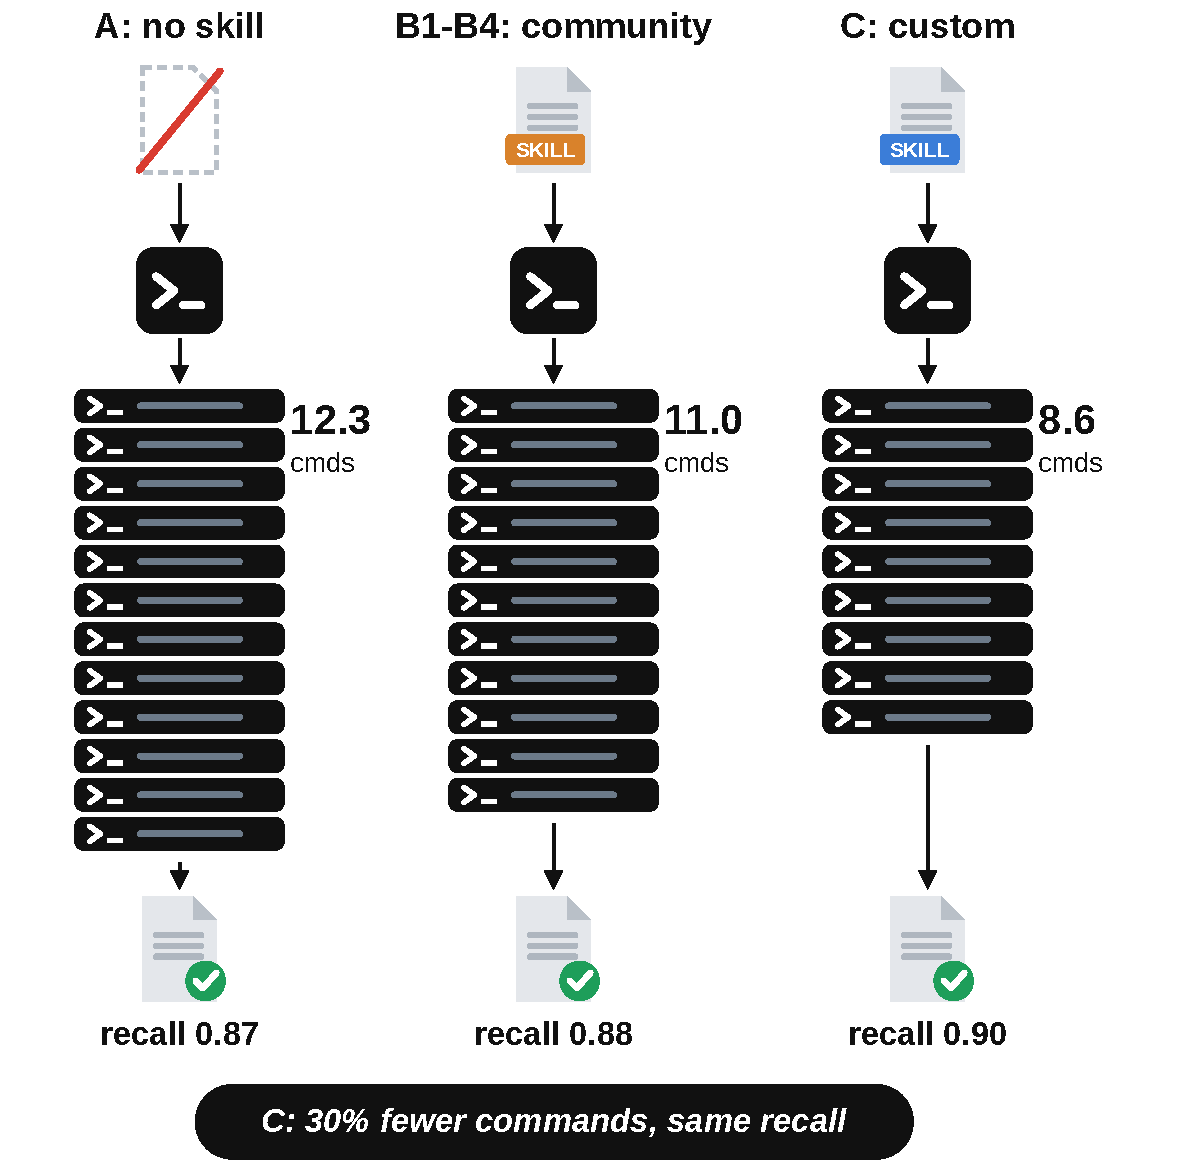
\includegraphics[width=\columnwidth]{../figures/fig_teaser.pdf}
\caption{Same agent, three skill conditions (primary model, Sonnet). Each chip is one
\texttt{tshark} command, drawn to the mean count per case; every condition reaches a report
with near-identical IOC recall.}
\label{fig:teaser}
\end{figure}

\noindent\textbf{Contributions.}
\begin{itemize}
\item A controlled nine-arm experiment design which isolates the contribution of a skill from the
contributions of its component parts using an LLM-agent network-forensics setup
(Section~\ref{sec:method}).
\item A validated nine-capture forensic benchmark with typed and evidence-checked ground truth
IOCs for RAT, stealer, and loader classes. Curation reveals a previously undiscovered
erroneous primary network indicator (C2 or victim IP and one victim MAC) in published answer
keys, which we corrected (Section~\ref{sec:dataset}).
\item Investigation of the influence of skill and component effects on the IOC recall,
attribution, hallucination, efficiency, and cost of the skill (Section~\ref{sec:results}).
The skill results in a statistically significant reduction in number of \emph{tool calls},
surviving multiple comparison adjustment and consistent across two models without any
decrease in accuracy and with indistinguishable faithfulness; we found that the skill effect
is localized to command recipes through the ablation study. We further introduce the
\emph{skill-issue effect}, where a specialized skill may constrain the exploration a
generalist agent would perform. This effect was discovered during piloting and addressed
during the experiment design phase (Section~\ref{sec:discussion}).
\item Open harness, data set, and skills corpus to support reproducibility.
\end{itemize}

\section{Related Work}

\subsection{LLM agents, reasoning, and tool use}
The large language models of today are all based on transformers~\cite{vaswani2017}.
In-context learning~\cite{brown2020} and instruction tuning~\cite{ouyang2022instructgpt}
allow one model to be steered via its prompt input. Chain-of-thought
prompting~\cite{wei2022cot} and self-consistency~\cite{wang2023selfconsistency} elicit
reasoning, which can be scaled with respect to model size~\cite{wei2022emergent}. Agency is
achieved through alternating between reasoning and action: ReAct~\cite{yao2023react} mixes
reasoning and calling of tools, Toolformer~\cite{schick2023toolformer} and
ToolLLM~\cite{qin2024toolllm} condition the model to call tools externally, and
Reflexion~\cite{shinn2023reflexion} brings self-critique into the mix. Evaluation has moved
beyond measuring just the accuracy of the final answer towards measuring the reasoning
process itself~\cite{tooltrajectories2025} and towards software tasks like
SWE-bench~\cite{jimenez2024swebench}. When looking at the problem in such terms, skills are
ways of conditioning a tool-using loop, and the key question is which parts of that
conditioning are decisive~\cite{tooluseevolution2026}.

\subsection{Agent Skills and procedural knowledge injection}
Agent Skills instantiate procedural knowledge (instructions, command recipes, output
contracts) into the generalist model at inference
time~\cite{anthropicskills2026,anthropicskills_blog,agentskillsio2026}. SkillsBench
benchmarks skills on a large suite of tasks and finds significant improvement, including in
cybersecurity~\cite{skillsbench2026}, whereas recent research conceives skills as an
institutional knowledge primitive~\cite{knowledgeactivation2026}. In both cases, a skill is
considered a whole, whereas we disassemble it. There is only a handful of contemporaneous
works which conduct either ablations or stress tests for agent skills, and they reach rather
discouraging results. Chacko et al.~\cite{whenskills2026} re-analyze a 180-run offensive CTF
experiment from the point of view of skill ablation and find no reliable increase in
accuracy. Huang~\cite{datascienceskills2026} deconstructs the structure of auto-generated
data-science skills and finds that the procedural overhead results in increased token
consumption without improving task performance. Wang et al.~\cite{notallskills2026} show, in
a variety of tasks, that a lot of skills do not help and may even harm. Our paper differs
from them in three aspects. Firstly, the domain is defense-oriented network/malware traffic
forensics, not CTF, data science, or generic tasks. In addition, the baseline consists of a
population of four widely adopted community skills rather than a single skill or an
auto-generated one, thus avoiding selection bias in the comparison. The reported cost
pertains to the agent's \emph{behavioral} cost and is captured by the number of tool calls
made, instead of the payload cost of skill content injection quantified via the data-science
ablation (a 4.5x increase in input tokens without any gains in accuracy). The axis of tool
calls is not a novel one: cost-aware evaluation of security agents is an active area of
research, and Kassianik et al.~\cite{costaware2026} argue that disciplined tool use is what
matters for the success of defensive-SOC agents. Reduced tool calls at a given accuracy is
not an entirely novel goal either; there is a whole efficiency literature that aims to do
so, and the Skill-to-LoRA~\cite{skilltolora2026} technique distills skills into adapters
precisely for the purpose of reducing the token cost per step. What our claims pertain to is
something more modest: in a fixed model-task-toolbox setting, a manually designed,
domain-matched \emph{prompt-injected} skill decreases tool calls as a by-product (\num{30}\%
fewer calls vs.\ no skill, replicated on two models), while none of the four community
skills significantly reduces tool calls on our primary model. This is consistent with the
data-science results regarding the token overhead: the two costs are distinct and can
co-exist, since skill injection still brings input tokens. We show that the behavioral cost
of a skill can decrease while its payload cost increases, depending on the quality of the
skill construction and its relevance to the domain. Structured output constraints are known
to reduce tool calling in open-weight models~\cite{constrainttax2026}, which is consistent
with the observation that removing an inflexible output schema does not harm performance.

\subsection{LLMs for cybersecurity and the SOC}
Today, LLM agents have applications in both offensive and defensive security
realms~\cite{agenticsecurity2025,securityduality2026}. Penetration testing surveys highlight
autonomous frameworks~\cite{pentestsurvey2026}, and critical analyses find hallucination,
especially flag hallucination, widespread across them~\cite{hackorhalluc2026}. The findings
are an impetus for evidence-based evaluation similar to what we propose in this paper.
Semi-autonomous solutions retain a human-in-the-loop feature~\cite{semiautopentest2025}. In
defense, there are knowledge-grounded agents~\cite{craken2025}, retrieval-enabled solutions
for novel threats~\cite{ragcyber2025}, and alert triage to alleviate SOC overload
problems~\cite{alertfatigue2026}. The closest work to our ablation study is Jang et
al.~\cite{airgappedir2026}, who develop a local LLM pipeline to analyze security incidents
and perform ablations of the pipeline components, namely removal of the orchestration layer
and deactivation of the verification module, the latter raising hallucination. We conduct
ablations of the skill components, keeping the agent architecture intact.
CyberSecEval~\cite{cyberseceval2024} and CyberSOCEval~\cite{cybersoceval2025} evaluate the
security capabilities of agents but do not investigate the skill mechanism.

\subsection{LLM agents for network forensics}
CyberSleuth~\cite{cybersleuth2026} is closest to our study: an autonomous blue-team agent
with a \texttt{tshark} sub-agent specialized in forensic analysis of web attacks.
Holmes~\cite{holmes2026} orchestrates tools for auditable DDoS attack investigation.
SIABench~\cite{handoverwheel2026} evaluates the security incident analysis capabilities of
LLM agents, including network forensics, using the scenarios created by blue-team training
platforms like CyberDefenders and a real-world test that includes the challenges offered by
the Malware-Traffic-Analysis.net website. TrafficLLM~\cite{trafficllm2025} adapts LLMs to
traffic representation, and GRIDAI~\cite{gridai2025} and IoT-traffic
agents~\cite{iotagent2025} are aimed at rule generation and interpretation. Overall, these
studies show that agents are capable of extracting forensic evidence from packet captures.
No work isolates and decomposes the skill mechanism, which is the main subject of our paper.

\subsection{Machine learning for network intrusion detection}
Traditionally, network defense was implemented via signature engines
(Suricata~\cite{suricata}, Zeek~\cite{zeek}), and nowadays machine learning classifiers are
being developed based on labeled flow data~\cite{cicids2017,idsdatasets2021}. The surveys
cover the field of deep learning IDS and dataset trends~\cite{idsdatasets2021}, and
controlled experiments on CIC-IDS2017~\cite{cicids2017eval2025} and imbalanced
datasets~\cite{mlnids2024} reveal high in-distribution accuracy. They classify the traffic
into attack and benign classes. Our agents give different outputs, namely a human-readable
incident report with grounded indicators, mapped to the adversary's
behavior~\cite{mitreattack2018}.

\subsection{Hallucination and faithfulness}
Hallucination, which is the claim by a model of content that lacks support from the source,
is one of the main failure modes of LLMs~\cite{ji2023hallucination,huang2025hallucination}.
In the context of forensics, this issue becomes especially significant because even a single
fabricated C2 indicator costs a lot of analysis effort or, alternatively, may lead to an
improper response. Therefore, fabricated indicators become a first-class metric in our
evaluation and are detected by retrieval-based grounding~\cite{lewis2020rag} against the
packet-capture data.

\section{Method}\label{sec:method}

\begin{figure*}[t]
\centering
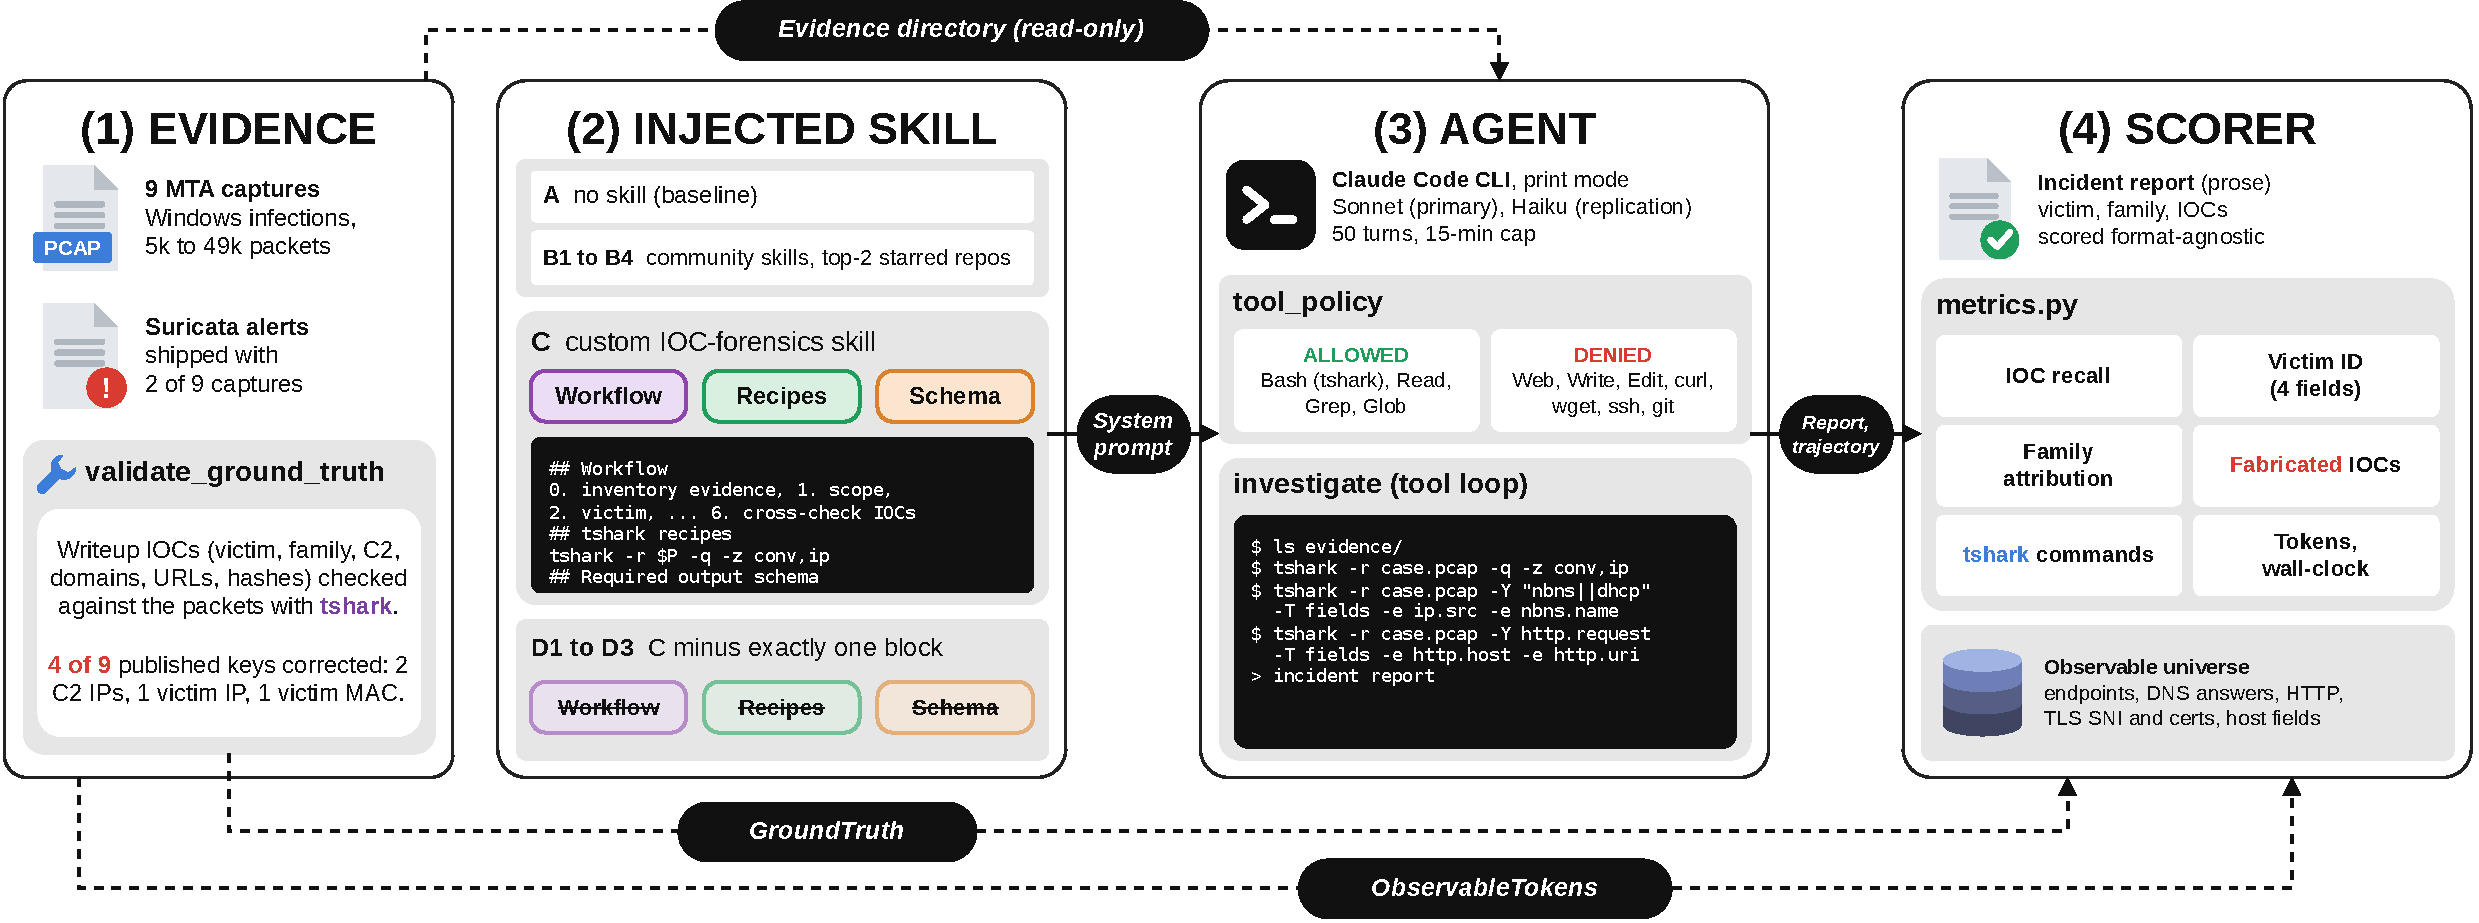
\includegraphics[width=\textwidth]{../figures/fig_architecture.pdf}
\caption{Evaluation architecture. Only the injected skill (2) varies across the nine arms;
the evidence (1), the agent and its read-only tool policy (3), and the scorer (4) are fixed.
D1--D3 each delete one block of the custom skill C. Input icons in Fig.~\ref{fig:scoring}: Microsoft Fluent Emoji
(MIT licence).}
\label{fig:schematic}
\end{figure*}

\subsection{The skill as independent variable}
In the described scenario, the agent runtime (Section~\ref{sec:setup}), the task prompt, and
the tool interface are held constant; the only parameter that changes is the injected skill.
Table~\ref{tab:arms} and Fig.~\ref{fig:schematic}(2) list the nine experimental conditions.
Arm~A is the control. To make sure that the ``community skill'' comparison does not rest on
one chosen skill (and to avoid cherry-picking), we test a \emph{population} of four
independent community skills (B1--B4). In addition, to confirm that the skills are used by
practitioners (and are not obscure or idiosyncratic), all four skills are taken from the two
most-starred public Claude-skill repositories (around \num{26}k and \num{30}k GitHub stars,
respectively, at the time of writing). B1--B3 were taken from the first repository and B4
from the second one; hence two different maintainers are involved. B2 is specifically
designed for malware traffic and is therefore the strongest community baseline for the
current task. Arm~C is the custom skill designed for this experiment. Arms~D1--D3 correspond
to arm~C with precisely one component removed; these arms are created programmatically by
removing a single marked section and differ from C by one component only.


\begin{table}[t]
\caption{The nine experimental arms. Only the injected skill differs. B1--B4 are a
population of independent, publicly-available community skills.}
\label{tab:arms}
\centering
\footnotesize
\setlength{\tabcolsep}{4pt}
\begin{tabular}{@{}lll@{}}
\toprule
Arm & Injected skill & Components present \\
\midrule
A  & none (vanilla)                       & n/a \\
B1 & community: Wireshark (repo~1)         & external \\
B2 & community: malware-traffic (repo~1)   & external \\
B3 & community: PCAP forensics (repo~1)    & external \\
B4 & community: Wireshark (repo~2)         & external \\
C  & custom IOC-forensics skill            & workflow + recipes + schema \\
D1 & C $-$ workflow                        & recipes + schema \\
D2 & C $-$ recipes                         & workflow + schema \\
D3 & C $-$ schema                          & workflow + recipes \\
\bottomrule
\end{tabular}
\end{table}

\begin{figure}[t]
\centering
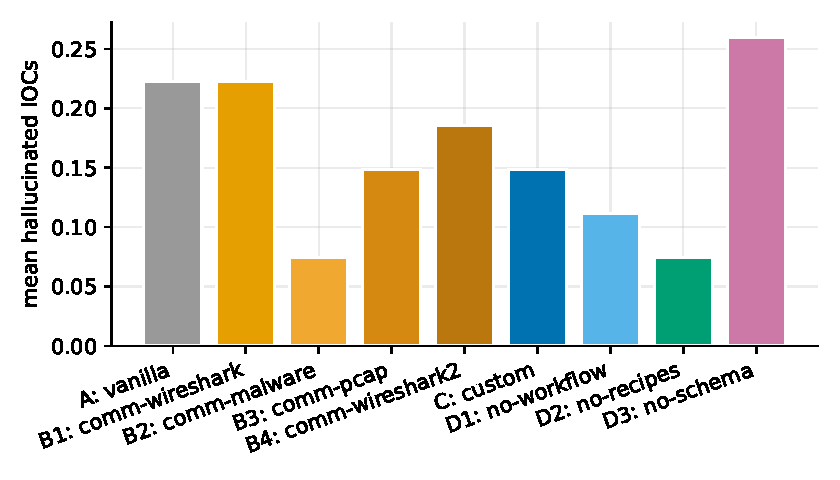
\includegraphics[width=0.92\columnwidth]{../figures/fig_halluc.pdf}
\caption{Mean fabricated indicators per case by arm. A fabricated indicator is an
IOC-shaped token the agent asserts that appears in zero packets. No community skill
(B1--B4) exceeds the baseline (B1 ties it at $0.22$), and no difference is significant at
$n{=}9$ (Table~\ref{tab:stats}).}
\label{fig:halluc}
\end{figure}

The custom skill (arm~C) consists of three separate components: (i) a \emph{procedural
workflow} describing the investigative process (evidence inventory, capture scoping, victim
identification, traffic shape determination, family attribution, and validation of each
indicator); (ii) \texttt{tshark} \emph{recipes} corresponding to the described procedures;
and (iii) a strict output \emph{schema} requiring a typed, evidence-annotated IOC set. Each
component has its own clearly identifiable section, and an ablation involves removal of one
section verbatim.

\begin{figure*}[t]
\centering
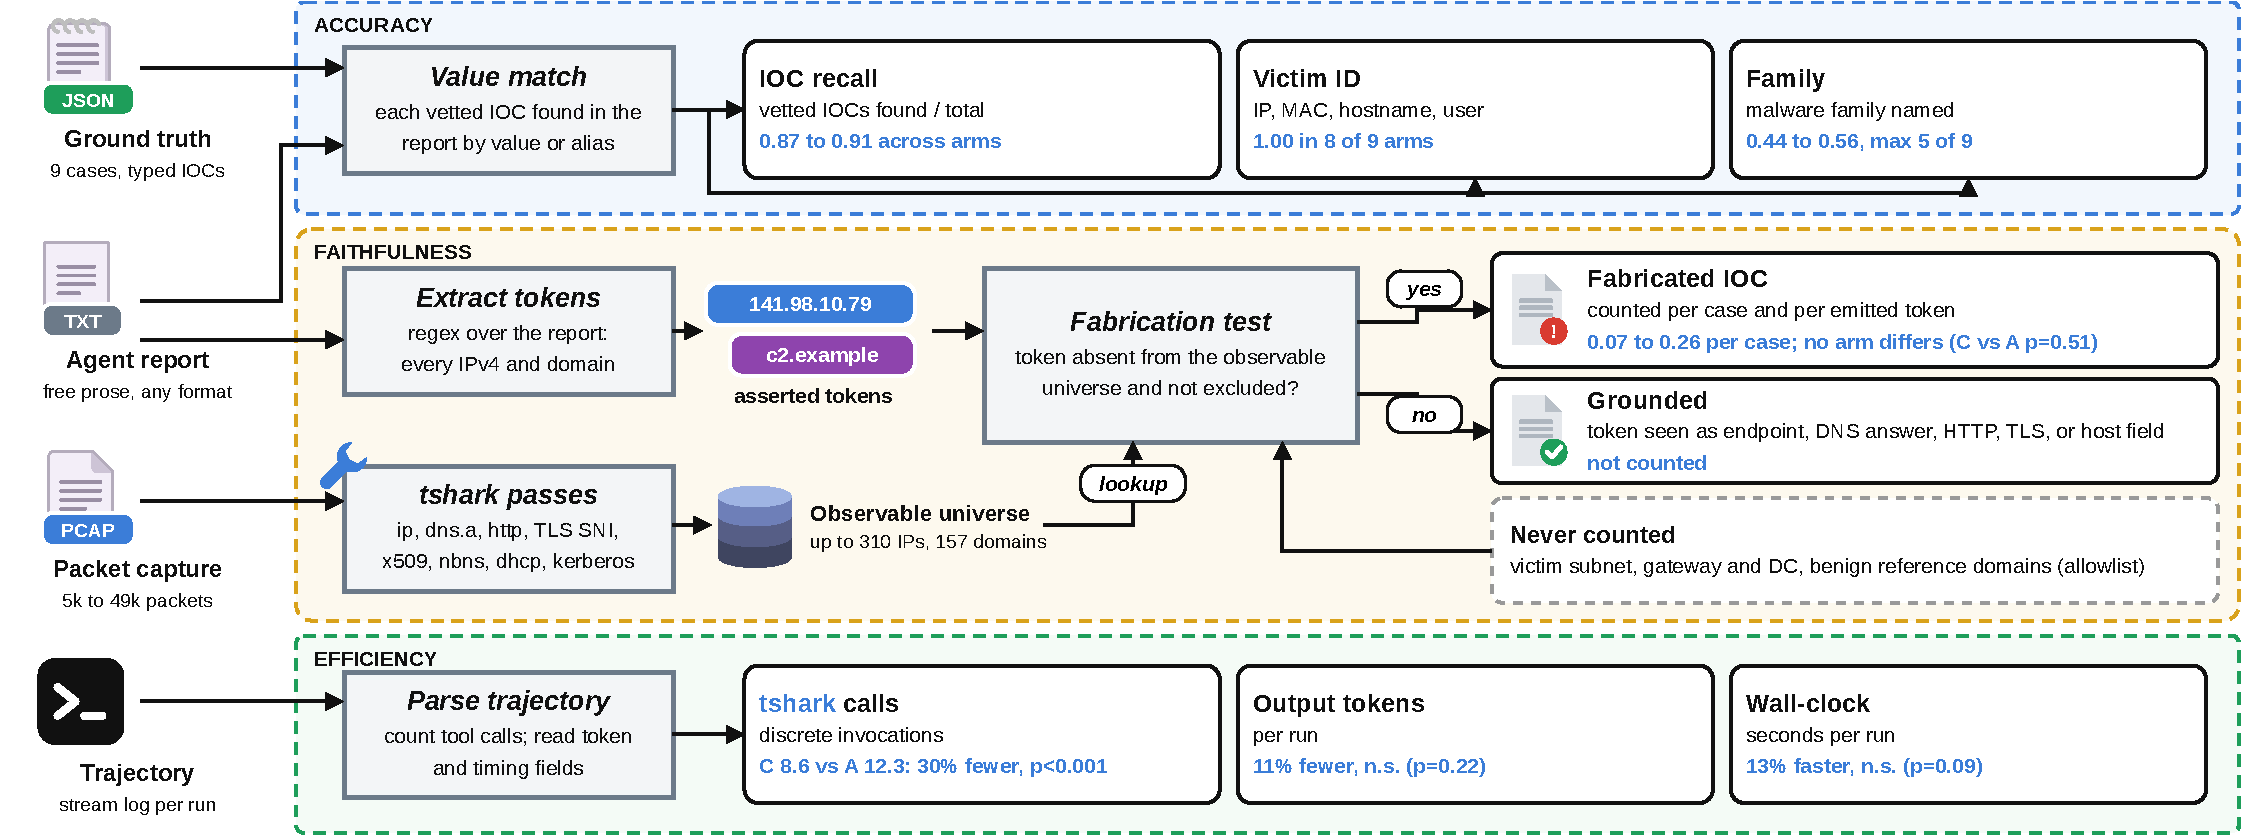
\includegraphics[width=\textwidth]{../figures/fig_scoring.pdf}
\caption{How a run is scored, in three lanes. Accuracy: each vetted IOC is matched by value
or alias in the prose report. Faithfulness: every IPv4 address and domain in the report is
tested against an observable universe built from \texttt{tshark} field passes, with local
infrastructure and benign reference domains never counted. Efficiency: tool calls, tokens,
and time come from the trajectory stream. Blue lines give the measured ranges (Sonnet).}
\label{fig:scoring}
\end{figure*}

\subsection{Task and scoring}
Every experimental condition comes with an identical neutral prompt: analyze the evidence
directory (consisting of a packet capture, possibly augmented with exported IDS alerts) and
write an incident report describing the victim host (IPv4 address, MAC address, hostname,
and user), the malware family, and all grounded IOCs. The prompt asks for a prose narrative,
so the schema ablation is not a source of bias, and scoring is agnostic to format. For every
run (Fig.~\ref{fig:scoring}), the following measurements are taken: \emph{IOC recall}
(fraction of vetted IOCs grounded in the report out of all vetted IOCs);
\emph{victim-identification accuracy} (four canonical fields); \emph{family attribution}
(correct vs.\ incorrect); \emph{hallucination count} (IOC-like entities claimed by the agent
and not present in the capture, measured against a per-capture universe of every observable
IP, domain, and host; this universe is constructed from packet endpoints, DNS queries
\emph{and answers}, HTTP hosts, request URIs, redirect and referer headers, TLS SNI and
certificate subject/SAN fields, and NetBIOS/DHCP/Kerberos host fields, excluding
local-subnet infrastructure and a documented benign-reference allowlist); \emph{tool-call
efficiency} (\texttt{tshark} calls); and \emph{cost} (output tokens, wall-clock time).

\subsection{Experimental setup}\label{sec:setup}
The agent executes inside the Claude Code CLI in non-interactive mode. The skill is
delivered as an appended system preamble, which separates procedural-knowledge
\emph{content} from skill-retrieval mechanics. The agent has access to read-only local
utilities (\texttt{tshark} through the shell, file reading, searching) and is forbidden from
accessing any web resources, file transfers, or writes to prevent any kind of solution
leakage; all trajectories are logged and audited for possible leaks. Every arm uses the same
model (Claude Sonnet) and follows the same constraints of \num{50} turns and a
\num{15}-minute wall-clock limit per run. The model is delivered as an unpinned alias, which
is a reproducibility constraint we acknowledge; exact bit-level replication requires pinning
down the build. The target is three repetitions per condition, and Section~\ref{sec:threats}
reports the coverage reached.

\section{Dataset}\label{sec:dataset}
The \num{9} real malware-infection packet captures are obtained from
Malware-Traffic-Analysis.net~\cite{mta}. They correspond to infections of an enterprise
Windows workstation and come with the official analyst write-up. Families of malware
involved include remote-access trojans (NetSupport RAT, NetSupport Manager RAT, STRRAT),
information stealers (Koi, Oski, Lumma, WarmCookie), and loaders (BazarLoader/TA551).
Capture size ranges from \num{5}k to \num{49}k packets. Two captures come with exported
Suricata alerts. The remaining seven cases require behavioral attribution.

\textbf{Ground-truth validation.} Transcription of each write-up resulted in a typed set of
IOCs (victim fields, family, C2 endpoints, domains, URLs, file names and hashes).
Subsequently, all network indicators were validated against their captures using
\texttt{tshark}. Validation revealed a wrong primary network indicator in \num{4} of \num{9}
exercises: the C2 IP address in two, the victim IP in one, and the victim MAC in one. In
each case, the value printed in the key did not match anything in any packet, while the
value on the actual port and session differed only slightly. For example, the STRRAT key
listed \texttt{141.98.10.69}, but the traffic on port 12132 was addressed to
\texttt{141.98.10.79}. All such values were fixed according to primary evidence and noted.
After validation, the victim IPs, C2 IPs, domains, and hostnames for all \num{9} cases
appear in their captures.

\section{Results}\label{sec:results}
Table~\ref{tab:main} reports the arm-level means per case: reps are averaged within a case,
then over the \num{9} cases, and the 95\% confidence intervals are in the released analysis
output. Table~\ref{tab:stats} reports the paired significance tests, which separate the
signal from the noise. To summarize: \textbf{the purpose-built skill provides a
statistically significant decrease in the number of tool calls per investigation, with no
significant change in accuracy or faithfulness.} The significant result is reported first,
followed by the null.

\subsection{The purpose-built skill significantly cuts discrete tool invocations}
\begin{figure}[t]
\centering
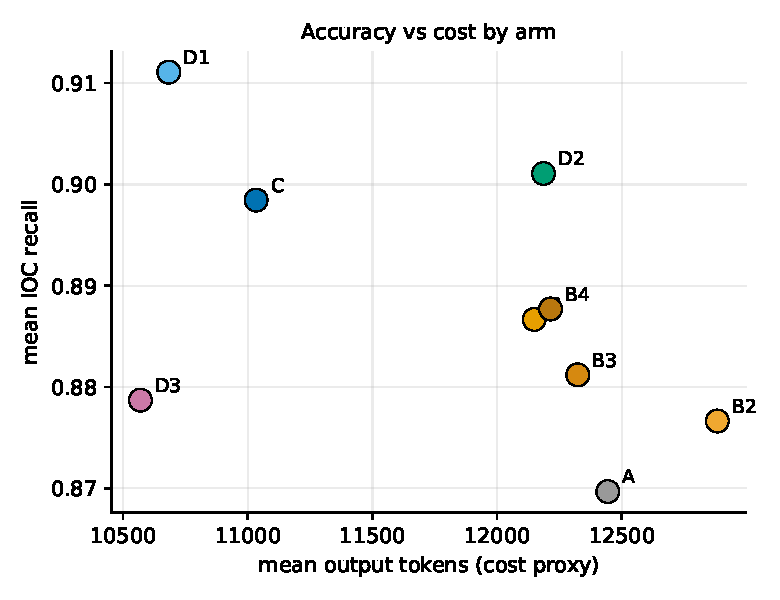
\includegraphics[width=0.86\columnwidth]{../figures/fig_pareto.pdf}
\caption{Accuracy versus cost. Each point is one arm's mean.}
\label{fig:pareto}
\end{figure}

This represents the main finding. Compared to the untreated baseline, the custom skill (C)
uses \num{30}\% fewer \texttt{tshark} invocations ($8.6$ vs $12.3$; paired $t{=}{-}5.14$,
$p{<}0.001$, $d_z{=}{-}1.71$), and compared to the four-skill community population, it uses
\num{22}\% fewer ($8.6$ vs $11.0$; paired $t{=}{-}7.14$, $p{<}0.001$, $d_z{=}{-}2.38$). The
community comparison does not change much without the toolbox-mismatched skill B4 ($21$\%,
$p{<}0.001$; Fig.~\ref{fig:community}, right). The effect is large and holds under pairing
in all \num{9} cases. A total of six cost comparisons were made, justifying a
Holm--Bonferroni correction on this family (Table~\ref{tab:stats}, adjusted $p$ in
parentheses); the reduction in tool invocations remains significant
($p_{\text{adj}}{=}0.005$). The paired differences form a small sample that might not be
normally distributed, so the non-parametric Wilcoxon signed-rank test confirms the result
($p{=}0.004$), with the effect size calculated using the Hedges small-sample correction
($g{=}{-}1.55$). The result does not depend on a normality assumption at $n{=}9$. There is
also a reduction in output tokens (\num{11}\%, $1.4$k fewer per case) and wall-clock time
(\num{13}\%), but neither change is significant on this model ($p{=}0.22$ and $p{=}0.09$,
respectively, and both drop out under correction). The interpretation is deliberately
conservative. The changed metric is the number of \emph{discrete} \texttt{tshark}
invocations; the token and wall-clock costs a SOC actually meters do not change
significantly at $n{=}9$. The parser treats each command as a single invocation irrespective
of the number of display fields and pipes it contains, which means that some of the effect
may be due to the skill batching work into fewer, richer commands rather than doing strictly
less. Thus, the conclusion is a smaller \emph{tool-invocation footprint}, rather than a
proven cost or latency advantage.

One may argue against the decreased command count in a rather straightforward manner by
pointing out that it simply reflects a decreased workload. However, the evidentiary yield
does not support such an interpretation. Mean counts of \emph{true} IOCs recovered do not
differ significantly between arms, and among the full-skill arms (A, B1--B4, C), C has the
highest count: $7.9$ compared to $7.7$ for the untreated baseline (out of $8.9$ possible per
case; two ablation arms recover marginally more). C reaches the same forensic results (the
identification of the victim and the same or a higher number of grounded indicators) with
fewer commands (Fig.~\ref{fig:pareto}) and devotes a larger fraction of those commands to
HTTP queries (Fig.~\ref{fig:grammar}).

\begin{figure}[t]
\centering
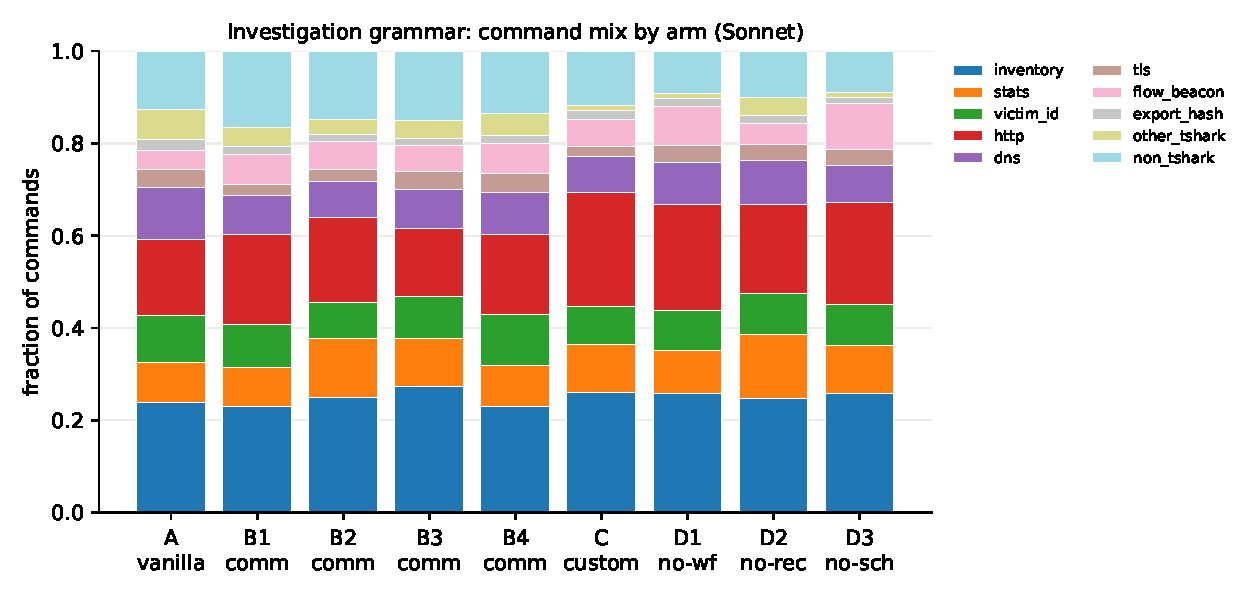
\includegraphics[width=\columnwidth]{../figures/fig_grammar.pdf}
\caption{Investigation grammar on the primary model (Sonnet): the share of each command
category per arm. The custom skill and its ablations spend a larger share on HTTP queries
and a smaller share on unclassified \texttt{tshark} and non-\texttt{tshark} commands than
the baseline and the community skills.}
\label{fig:grammar}
\end{figure}

\subsection{Accuracy and faithfulness: no significant difference}
\begin{figure}[t]
\centering
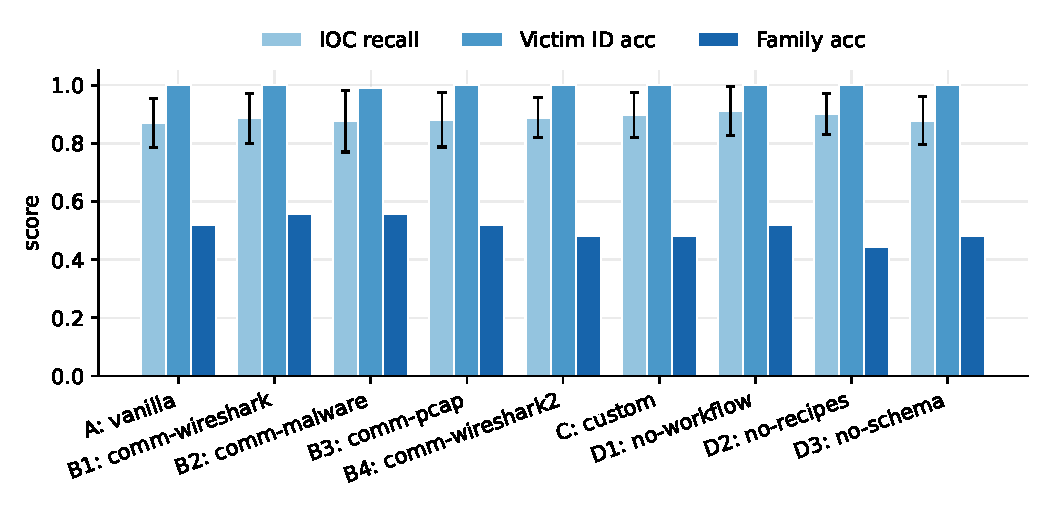
\includegraphics[width=\columnwidth]{../figures/fig_main_bars.pdf}
\caption{IOC recall, victim-ID accuracy, and family attribution by arm.}
\label{fig:main}
\end{figure}

No arm differs from the baseline significantly with respect to any measure of accuracy
(Table~\ref{tab:stats}, Fig.~\ref{fig:main}). Victim identification is close to perfect,
with $1.00$ achieved in all arms apart from the malware-specific community skill B2 ($0.99$,
due to missing one field in a single run). IOC recall falls in a narrow band of only
$0.87$--$0.91$, and the difference between C and A is not statistically significant (the
custom skill is nominally better by $0.03$, $p{=}0.08$). A two-one-sided-tests (TOST)
equivalence check at a $\pm0.05$ margin is marginal ($p{=}0.09$; equivalence is established
only for margins of about $\pm0.056$ or more). Therefore, recall is reported as a
non-significant difference in favor of the skill rather than a formally demonstrated
equivalence. In any case, no skill \emph{reduces} recall, and the 95\% confidence intervals
of all nine arms overlap.

Faithfulness shows no observable effect either. Fabrication is judged based on absence from
a per-capture ``universe'' of observable tokens: packet endpoints, DNS query \emph{and
answer} records, HTTP hosts and request URIs, TLS SNI and certificate names, and
NetBIOS/host fields (Section~\ref{sec:method}). The universe deliberately gives credit for
payload-based indicators that a diligent analyst would legitimately report. Under this
stringent scoring, fabrication is uniformly low ($0.07$--$0.26$ indicators per case;
Fig.~\ref{fig:halluc}), with no arm showing a significant difference from any other arm. The
custom skill ($0.15$) does not differ from the untreated baseline ($0.22$, $p{=}0.51$), and
the community skills vary between $0.07$ and $0.22$. Under a laxer universe, an initially
favorable faithfulness effect appeared for the custom skill, but it disappears when the
universe includes DNS-answer and payload fields, so we report the null. A secondary,
length-normalized view agrees with the finding. As a \emph{rate} over emitted IOC tokens,
the custom skill ($0.011$) is lower than the untreated baseline ($0.019$), but with the
counts null, it is not claimed as a result. The metric has an inherent limitation: it
detects only gross fabrication. The universe is large (up to \num{310} IPs and \num{157}
domains in the busiest capture) and domain matching is done by suffix; hence a fabricated
indicator that resembles an observed one can slip through. The null result means ``no arm
grossly fabricates,'' not that fabrication is zero. Family attribution is between $0.44$ and
$0.56$ for all arms and varies by at most one case between arms; one capture has no labeled
ground-truth family and is thus rated unattributed for all arms, with blanks scored
incorrect.

As a result, both accuracy and faithfulness are nulls: no injected skill moves recall,
victim identification, or fabrication. Skills differ in tool-call cost. The custom skill
calls significantly fewer \texttt{tshark} commands than the community population under
\emph{both} models: $8.6$ vs $11.0$ on Sonnet (paired $p{<}0.001$) and $20.1$ vs $27.5$ on
Haiku ($p{<}0.001$). This difference from real, widely used community skills is the result
that holds on both models.

\begin{figure}[t]
\centering
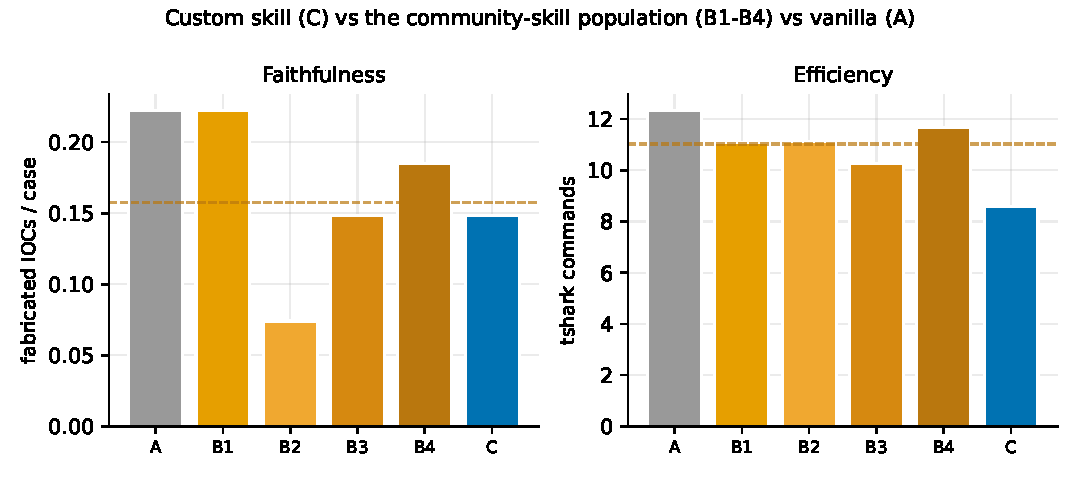
\includegraphics[width=\columnwidth]{../figures/fig_community.pdf}
\caption{The custom skill (C) against the four-skill community population (B1--B4) and
the untreated baseline (A). C issues the fewest \texttt{tshark} commands of any skill
shown, its one significant advantage. Under strict evidence-grounded scoring, fabrication
is low and statistically indistinguishable across arms. The dashed line marks the
community-population mean, so the comparison rests on a population of widely adopted
skills rather than a single baseline.}
\label{fig:community}
\end{figure}

\begin{table*}[t]
\caption{Per-arm results on the primary model (Sonnet), case-level mean over \num{9}
cases. B1--B4 form the community-skill population. Recall, victim, and family are
fractions; hallucination is fabricated IOCs per case (lower is better); \texttt{tshark} is
the mean command count; tokens are mean output tokens. Among the full skills (A--C), the
custom skill (C) issues the fewest \texttt{tshark} commands with no significant recall
difference, and fabrication is low and statistically indistinguishable across all arms.}
\label{tab:main}
\centering
\footnotesize
\begin{tabular}{@{}lrrrrrr@{}}
\toprule
Arm & Recall & Victim & Family & Halluc.$\downarrow$ & \texttt{tshark}$\downarrow$ & Tok$\downarrow$ \\
\midrule
A: vanilla & 0.870 & 1.000 & 0.52 & 0.22 & 12.3 & 12444 \\
B1: comm-wireshark & 0.887 & 1.000 & 0.56 & 0.22 & 11.1 & 12149 \\
B2: comm-malware & 0.877 & 0.991 & 0.56 & 0.07 & 11.1 & 12884 \\
B3: comm-pcap & 0.881 & 1.000 & 0.52 & 0.15 & 10.3 & 12324 \\
B4: comm-wireshark2 & 0.888 & 1.000 & 0.48 & 0.19 & 11.7 & 12215 \\
\midrule
\textbf{C: custom} & \textbf{0.898} & 1.000 & 0.48 & 0.15 & \textbf{8.6} & 11034 \\
D1: no-workflow & 0.911 & 1.000 & 0.52 & 0.11 & 9.1 & 10683 \\
D2: no-recipes & 0.901 & 1.000 & 0.44 & 0.07 & 9.9 & 12186 \\
D3: no-schema & 0.879 & 1.000 & 0.48 & 0.26 & 9.3 & 10569 \\
\bottomrule
\end{tabular}
\end{table*}

\begin{table*}[t]
\caption{Paired $t$-tests across the \num{9} cases ($\Delta$ = arm minus comparator;
$d_z$ = paired effect size; the parenthesized $p$ and the significance stars are
Holm-adjusted over the six cost contrasts). Only the tool-call reduction (C$-$A) is
significant; its effect is large and survives correction. The token and wall-clock
reductions point the same way without reaching significance, and no accuracy contrast is
significant. ***$p{<}.001$, **$p{<}.01$, *$p{<}.05$.}
\label{tab:stats}
\centering
\footnotesize
\begin{tabular}{@{}llrrrrl@{}}
\toprule
Metric & Contrast & $\Delta$ & $t$ & $p$ & $d_z$ & sig \\
\midrule
\multicolumn{7}{@{}l}{\emph{Efficiency / cost}}\\
tshark calls & C$-$A & -3.74 & -5.14 & $<$0.001 (0.005) & -1.71 & \textbf{**} \\
tshark calls & B1$-$A & -1.26 & -1.30 & 0.230 (0.899) & -0.43 & ns \\
output tokens & C$-$A & -1410.67 & -1.32 & 0.225 (0.899) & -0.44 & ns \\
output tokens & B1$-$A & -294.96 & -0.22 & 0.831 (1.000) & -0.07 & ns \\
wall time s & C$-$A & -25.37 & -1.91 & 0.093 (0.465) & -0.64 & ns \\
wall time s & B1$-$A & -4.58 & -0.24 & 0.817 (1.000) & -0.08 & ns \\
\midrule
\multicolumn{7}{@{}l}{\emph{Accuracy / faithfulness}}\\
recall & C$-$A & +0.03 & 2.00 & 0.081 & +0.67 & ns \\
hallucination count & C$-$A & -0.07 & -0.69 & 0.512 & -0.23 & ns \\
fam & C$-$A & -0.04 & -1.00 & 0.347 & -0.33 & ns \\
\bottomrule
\end{tabular}
\end{table*}

\subsection{Component ablation}
\begin{figure}[t]
\centering
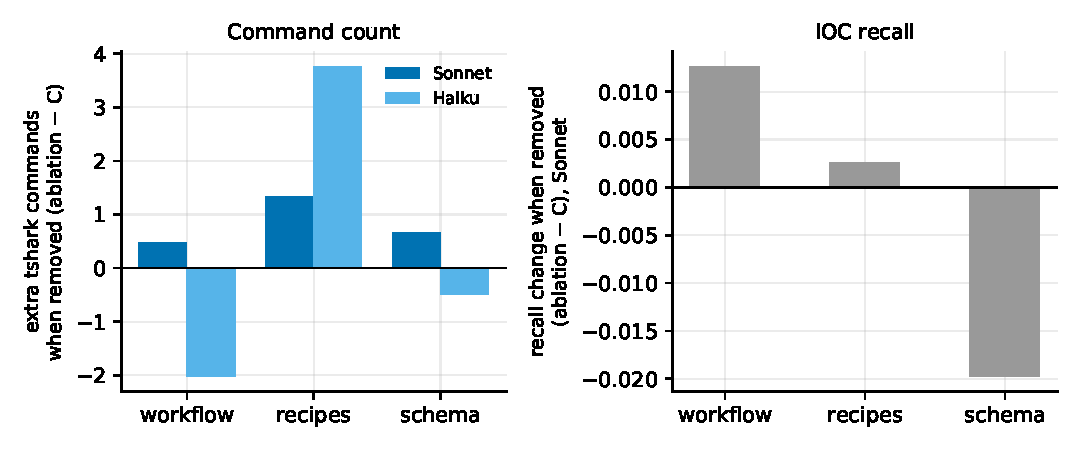
\includegraphics[width=0.9\columnwidth]{../figures/fig_ablation.pdf}
\caption{Effect of removing each component, computed as the ablation minus the full
skill (C), case-level means. Left: extra \texttt{tshark} commands on both models; only
removing the recipes adds commands on both. Right: change in IOC recall on Sonnet; all
three changes are within $\pm0.02$ and none is significant.}
\label{fig:ablation}
\end{figure}

Ablating the components of the custom skill one by one (arms D1--D3) tests what accounts for
the tool-call reduction (Fig.~\ref{fig:ablation}). In terms of accuracy and faithfulness,
the ablations, like the main arms, do not produce any noticeable effects: recall
($0.88$--$0.91$), family attribution ($0.44$--$0.52$), and fabrication ($0.07$--$0.26$) stay
within noise level, and none of the single-component differences stays significant after
correction at $n{=}9$. Ablating the \emph{workflow} (D1) does not reduce recall or
attribution on the clean data; both values are nominally slightly higher with the ablation.
Hence, we withdraw the more confident interpretation, derived from our previous mixed-epoch
data, that the workflow drives accuracy. All ablations agree on the \emph{command count}.
The complete skill (C) shows the smallest command usage ($8.6$), while each ablation
generates more commands (no-workflow $9.1$, no-schema $9.3$, no-recipes $9.9$). The
exclusion of the \texttt{tshark} \emph{recipes} comes with the largest price: the difference
between C and D2 is $+1.3$ commands and is nominally significant ($p{=}0.02$ uncorrected)
but not after correction. The Haiku replication confirms this pattern
(Fig.~\ref{fig:ablation}, left). Without the recipes, the agent again issues the largest
number of commands ($23.8$ vs $20.1$, $+3.8$, $p{=}0.09$), but without the workflow ($18.0$,
$p{=}0.18$) or the schema ($19.6$, $p{=}0.33$), the Haiku agent is \emph{leaner} than with
the full skill. Hence, the recipes are the only component of the skill whose ablation
increases the command count in both models. The effects of the workflow and schema change
direction between models, and we make no claim for them. The output \emph{schema} remains
neutral along all dimensions. Omitting it changes neither recall nor fabrication
significantly; in fact, D3 fabricates nominally \emph{more} than C ($0.26$ vs $0.15$),
further weakening any ``the schema pressures fabrication'' interpretation. The ablation
should be treated as a ranking by directional impact on tool usage, and it leads to one
conclusion: invest in concrete command recipes rather than a rigid output template.

\subsection{Attribution is the hard ceiling}
The maximum attainable level of family attribution for each arm is \num{5} of \num{9} cases.
The families missed every time (Oski Stealer, WarmCookie, BazarLoader, and the
fake-authenticator infostealer) coincide with cases where there are no IDS alerts and the
family has to be derived from traffic alone. In all cases where Suricata alerts are present,
each arm uses them and attributes correctly; without them, no skill bridges the gap. This
puts a bound on what can be accomplished with packet-only agentic attribution.

\subsection{Cross-model replication (Haiku)}
To check whether the results are due to skills or to a particular model, the full nine-arm
protocol was repeated using a smaller model (Claude Haiku), with three repeats per case,
resulting in \num{239} valid runs (Table~\ref{tab:crossmodel}). The reduction in tool calls
is confirmed and is the only contrast significant on \emph{both} models: the custom skill
cuts \texttt{tshark} commands by \num{35}\% on Haiku (paired $t{=}{-}5.39$, $p{<}0.001$,
$d_z{=}{-}1.80$), compared to \num{30}\% on Sonnet. The output-token reduction is
significant on Haiku (\num{11}\%, $p{=}0.027$) but not on Sonnet ($p{=}0.22$). Wall-clock
reductions are not significant on either model ($p{=}0.09$ on Sonnet, $p{=}0.31$ on Haiku);
per-run wall-clock variability is substantial, and a single slow run can heavily skew the
average per case. For both models, the consistent outcome is a reduced \emph{command count},
not a uniform token or latency win.

As far as accuracy goes, the full Haiku dataset erases a trend seen in a single repetition.
There is virtually no difference in IOC recall between the vanilla and custom configurations
($p{=}0.97$), while the improvement in victim ID from $0.88$ to $0.96$ is not statistically
significant ($p{=}0.08$). The ``weak model gains accuracy'' trend seen in rep~1 was just
noise. Both models arrive at the same conclusion: a skill changes tool-call cost but does
not improve correctness.

\begin{table*}[t]
\caption{Cross-model comparison of vanilla (A) and the custom skill (C), case-level means
(Sonnet and Haiku, three reps each). The tool-call reduction is significant on both
models. The token reduction is significant on Haiku only, and the wall-clock reduction on
neither; Haiku A's wall-clock is inflated by a few slow runs ($p{=}0.31$). Accuracy does
not differ on either model.}
\label{tab:crossmodel}
\centering
\footnotesize
\begin{tabular}{@{}llrrrrr@{}}
\toprule
Model & Arm & Recall & Victim & Halluc.$\downarrow$ & \texttt{tshark}$\downarrow$ & Wall s$\downarrow$ \\
\midrule
Haiku & A & 0.776 & 0.880 & 0.19 & 30.8 & 447 \\
 & C & 0.778 & 0.963 & 0.15 & 20.1 & 151 \\
\midrule
Sonnet & A & 0.870 & 1.000 & 0.22 & 12.3 & 188 \\
 & C & 0.898 & 1.000 & 0.15 & 8.6 & 163 \\
\bottomrule
\end{tabular}
\end{table*}

\subsection{Per-case detail and error analysis}
Table~\ref{tab:percase} gives the complete per-case grid, and Fig.~\ref{fig:heatmap} its
heatmap representation. Recall stays at ceiling or close to it for most of the captures; the
dispersion among arms is due to some hard cases, not to any general shift. Two types of
errors are seen repeatedly, and concrete examples of them follow.

\emph{Fabrication.} On the Lumma capture, one IPv4 address (\texttt{172.56.88.98}) was
reported by arm~C as a C2 endpoint, although it was never observed in any packet, neither as
a frame endpoint nor as a DNS answer. Under a less restrictive universe without DNS answers,
the same run scored four fabrications, three of which were legitimate resolved addresses;
this is why the universe was completed and the runs re-scored. On this capture, the
no-schema arm (D3) left the field empty, but this pattern does not generalize. D3 showed
fabrication on two other captures where C does not, meaning that fabrication cannot be
considered a schema effect (Section~\ref{sec:results}).

\emph{Suppressed exploration (the skill-issue effect).} At an early stage, in the presence
of the custom skill's \texttt{tshark}-centered recipes, the agent went straight to the
capture, omitting the enumeration of the evidence directory and hence the IDS alert file
naming the family, while the untreated agent explored and opened the directory. An explicit
evidence-inventory step in the workflow counteracted the effect. In the final dataset, every
arm, including the no-workflow ablation, opened the IDS alert file in all \num{6}
alert-bearing runs.

\begin{table*}[t]
\caption{Per-case IOC recall for arms A, B1, and C, the standard deviation of recall
across those arms, and arm~C's hallucination and \texttt{tshark} count. Most cases sit near
ceiling, and the spread is concentrated in a few hard captures.}
\label{tab:percase}
\centering
\footnotesize
\begin{tabular}{@{}lrrrrrr@{}}
\toprule
 & \multicolumn{3}{c}{IOC recall} & \multicolumn{3}{c}{Halluc.\ / tshark (C)} \\
\cmidrule(lr){2-4}\cmidrule(lr){5-7}
Case & A & B1 & C & rec.\ sd & hal.\ C & tshk C \\
\midrule
2021-09-10 & 0.83 & 0.90 & 0.90 & 0.04 & 0.0 & 8 \\
2022-01-07 & 0.89 & 0.89 & 0.89 & 0.00 & 0.0 & 7 \\
2024-07-30 & 0.78 & 0.78 & 0.78 & 0.00 & 0.3 & 8 \\
2024-08-15 & 0.76 & 0.85 & 0.79 & 0.05 & 0.0 & 9 \\
2024-09-04 & 0.89 & 0.89 & 0.89 & 0.00 & 0.0 & 8 \\
2024-11-26 & 0.96 & 0.93 & 1.00 & 0.04 & 0.0 & 7 \\
2025-01-22 & 0.79 & 0.75 & 0.92 & 0.09 & 0.7 & 10 \\
2026-01-31 & 0.93 & 1.00 & 0.93 & 0.04 & 0.0 & 11 \\
2026-02-28 & 1.00 & 1.00 & 1.00 & 0.00 & 0.3 & 9 \\
\bottomrule
\end{tabular}
\end{table*}

\begin{figure}[t]
\centering
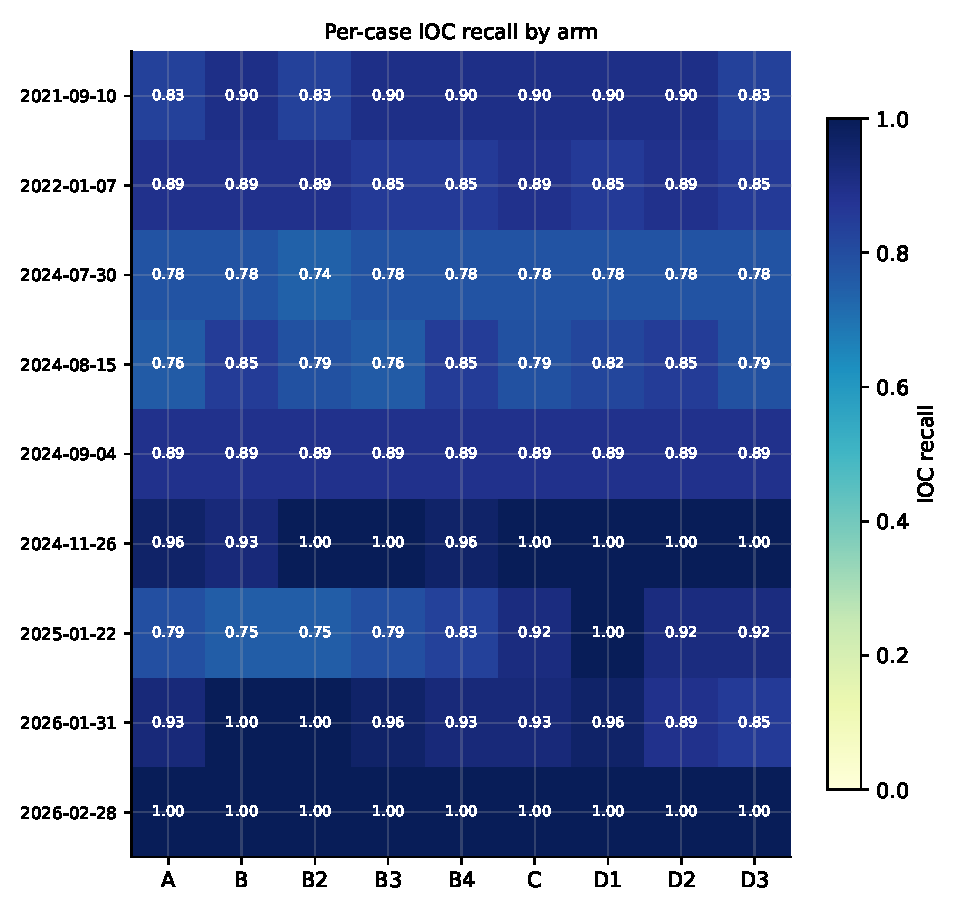
\includegraphics[width=\columnwidth]{../figures/fig_heatmap.pdf}
\caption{Per-case IOC recall by arm.}
\label{fig:heatmap}
\end{figure}


\section{Discussion}\label{sec:discussion}
\textbf{Given a strong base model, skills serve as efficiency utilities for the agent, not
as capability or safety enhancements.} The return on a network-forensics skill built on a
capable model is therefore a leaner \emph{tool-use footprint}, not an improved accuracy
ceiling or measurably fewer fabrications. The leaner footprint is a real saving: a
\num{30}\% reduction in tool calls without any significant recall difference, replicated on
two models and significant even after correction for multiple comparisons, matters in a SOC
environment where tool invocations are metered. Reductions in token usage and wall-clock
time are consistent with this trend but fail to reach significance at $n{=}9$; no latency
advantage can therefore be claimed. Teams expecting a skill to lift a weak model to
competence or to make a good model more truthful must measure, not assume.

\textbf{There are limits to the utility of the output schema.} Component-level ablation
isolates the areas in which effort expended in skill authoring bears fruit. Removing the
strict typed-IOC output schema preserved recall and, with strict evidence-based scoring, a
similar fabrication rate; thus, on this task the output schema shows no measurable benefit.
One methodological note concerning our approach: with less strict scoring criteria, the
schema initially appeared to \emph{increase} fabrication, but the effect disappeared upon
adding DNS-answer and payload fields. Faithfulness metrics rely on the correctness of the
observability model behind them. Skill authors would find concrete command recipes more
useful than an inflexible output schema. Where an output schema is used, the statement ``no
indicator of this type was observed'' must be treated as a first-class answer.

\textbf{Skill-issue effect.} In the pilot failure outlined in Section~\ref{sec:results}, the
\texttt{tshark}-centric recipes blocked the agent from inspecting the evidence directory and
cost it a family attribution that the unaltered baseline made. The narrow focus of a skill
may prevent the exploration typical of a generalist agent. The larger point is that a skill
must expand, not limit, the evidentiary space inspected by an agent.

\section{Threats to Validity}\label{sec:threats}
All ground-truth data have only one source (MTA); evidence validation per capture and
malware-family diversity mitigate this limitation. The skill was incorporated into the
experiment as a system preamble rather than through the native skill loader, thereby
separating content from retrieval; effects related to the native skill loader will be
addressed in future work. The efficiency effect replicates on another model (Haiku);
generalization to more vendors will be part of future research. At $n{=}9$, differences
between conditions in terms of accuracy and faithfulness are underpowered compared to
case-level variance (recall sd $\approx$\num{0.08}; fabrication has low values, sd
\num{0.15}--\num{0.36}); therefore, they are reported as nulls rather than claims. The one
effect that is large, survives multiple-testing correction, and holds across models is the
tool-call reduction. We collected three repetitions per condition across all nine arms and
two models (\num{482} valid runs: \num{243} Sonnet, \num{239} Haiku). For the primary model,
all nine arms were re-collected in a \emph{single continuous batch}, with three repetitions
for each of the \num{9} cases and \num{9} arms. In this way, we eliminate the
collection-epoch confound that existed in a previous version of this dataset collected in
mixed batches, because all cross-arm contrasts now fall within one epoch. Data for the
secondary model (Haiku) were collected in one batch as well. The model is an unpinned alias,
which is a reproducibility limitation we acknowledge. However, each batch spanned no more
than a few days; thus residual build drift is small but not provably zero, and exact
bit-level replication would require exact build pinning.

The custom skill itself is a further limitation. Its workflow was refined after a failure on
one evaluation capture; hence arm~C was not developed on a held-out set. The ablation
contrasts (C versus its constituent components) are internal to the skill and are not
affected by this, and the efficiency effect replicates on another model. Still, the standing
of C relative to the community skills could be somewhat optimistic for this reason; a blind,
held-out evaluation of a frozen skill will be future work.

\section{Conclusion}
We divide the deployment of procedural knowledge for LLM-agent network forensics into a
nine-arm experiment. In the case of a good base model, a custom skill improves tool-use
efficiency but not accuracy or faithfulness. Our method reaches identical conclusions
through the use of far fewer commands (\num{30}\% reduction when compared to using no skill
at all, $p{<}0.001$, replicated on a second model), while not compromising recall and with
fabrication indistinguishable across arms. In the component ablation, concrete command
recipes emerge as the only component whose absence results in more commands for both
models, while the influence of workflow and schema is inconsistent across models. Command
recipes should be prioritized by skill developers over output templates, and skills should
be created in such a way as to expand the scope of evidence used by the agent. The harness,
the evidence-validated dataset, and all skill
variants\footnote{\url{https://github.com/yaakulya123/skill-issue-pcap-forensics}} are
released for replication and extension.

\bibliographystyle{IEEEtran}
\bibliography{refs}
\end{document}
